\subs{MEGA(门控移动平均注意力)}
\label{subsec:mega}

在本节中,我们介绍 ~\cite{ma2023mega} 提出的门控移动平均注意力(Moving Average Equipped Gated Attention,MEGA)方法。
我们将首先介绍多维阻尼指数移动平均(Multi-dimensional Damped EMA)(\ref{subsubsec:mddema}),和门控注意力层(\ref{subsubsec:mega})。接下来,我们引入 MEGA-chunk 将输入序列进行固定大小的分块,从而将序列处理的复杂性从平方降低到线性(\ref{subsec:mega-chunk})。

\subsubs{多维阻尼指数移动平均}
\label{subsubsec:mddema}

MEGA 引入了一种改进的标准指数移动平均(EMA)方法,称为多维阻尼指数移动平均。~\cite{svetunkov2016complex}指出,通过减小先前元素和当前元素间的关联权重($\boldsymbol{\alpha}$ 和 \eqref{eq:ema} 中的 $1 - \boldsymbol{\alpha}$),可以实现稳健的依赖建模。受此启发,MEGA 在经典的EMA中引入阻尼因子,从而允许模型减小先前时间步元素的权重:
\begin{equation}
\label{eq:damping}
\mathbf{y}_t = \boldsymbol{\alpha} \odot \mathbf{x}_t + (1 - \boldsymbol{\alpha} \odot \boldsymbol{\delta}) \odot \mathbf{y}_{t-1},
\end{equation}
其中 $\boldsymbol{\delta} \in (0, 1)^{d}$ 是阻尼因子。

为了进一步增强 EMA 的表示能力,MEGA 设计了多维阻尼移动平均机制。首先,通过扩展矩阵 $\boldsymbol{\beta} \in \mathbb{R}^{d\times h}$ 将输入序列 $\boldsymbol{X}$ 的每个维度的标量单独扩展到 $h$ 维。对于每个维度的标量 $j \in \{1, 2, \ldots, d\}$:
\begin{equation}
\mathbf{u}^{(j)}_t = \boldsymbol{\beta}_j \mathbf{x}_{t,j}
\end{equation}
其中 $\boldsymbol{\beta}_j \in \mathbb{R}^{h}$ 是 $\boldsymbol{\beta}$ 的第 $j$ 行,  $\mathbf{u}^{(j)}_t \in \mathbb{R}^{h}$ 是第 $j$ 维在时间步 $t$ 展成的 $h$ 维向量.

相应地,我们将$\boldsymbol{\alpha}$和$\boldsymbol{\delta}$的形状从一维向量扩展为二维矩阵,即$\boldsymbol{\alpha}$,$\boldsymbol{\delta} \in \mathbb{R}^{d\times h}$,其中$\boldsymbol{\alpha}_j$,$\boldsymbol{\delta}_j \in \mathbb{R}^{h}$ 分别表示$\boldsymbol{\alpha}$和$\boldsymbol{\delta}$的第$j$行。
然后,对于每个维度$j$,在$h$维隐空间上应用阻尼EMA:
\begin{align}
\label{eq:mddema}
\mathbf{h}^{(j)}_t & = \boldsymbol{\alpha}_j \odot \mathbf{u}^{(j)}_t + (1 - \boldsymbol{\alpha}_j \odot \boldsymbol{\delta}_j) \odot \mathbf{h}^{(j)}_{t-1} \nonumber \\
\mathbf{y}_{t,j} & = \boldsymbol{\eta}^T_j \mathbf{h}^{(j)}_t
\end{align}
其中$\mathbf{h}^{(j)}_t \in \mathbb{R}^{h}$ 是时间步$t$时第$j$维度的EMA隐藏状态。
$\boldsymbol{\eta} \in \mathbb{R}^{d\times h}$ 是投影矩阵,将$h$维隐藏状态映射回$1$维输出$\mathbf{y}_{t,j} \in \mathbb{R}$。$\boldsymbol{\eta}_j \in \mathbb{R}^{h}$ 是$\boldsymbol{\eta}$的第$j$行。
从\eqref{eq:mddema}中得到的输出$\boldsymbol{Y}$被表示为$\boldsymbol{Y} \stackrel{\Delta}{=} \mathrm{EMA}(\boldsymbol{X})$。
由于不需要显式计算 $\mathbf{h}^{(j)}_t$ 来获取输出 $\mathbf{y}_{t,j}$,时间和空间复杂度与标准EMA相似。

\begin{figure}[!t]
\centering
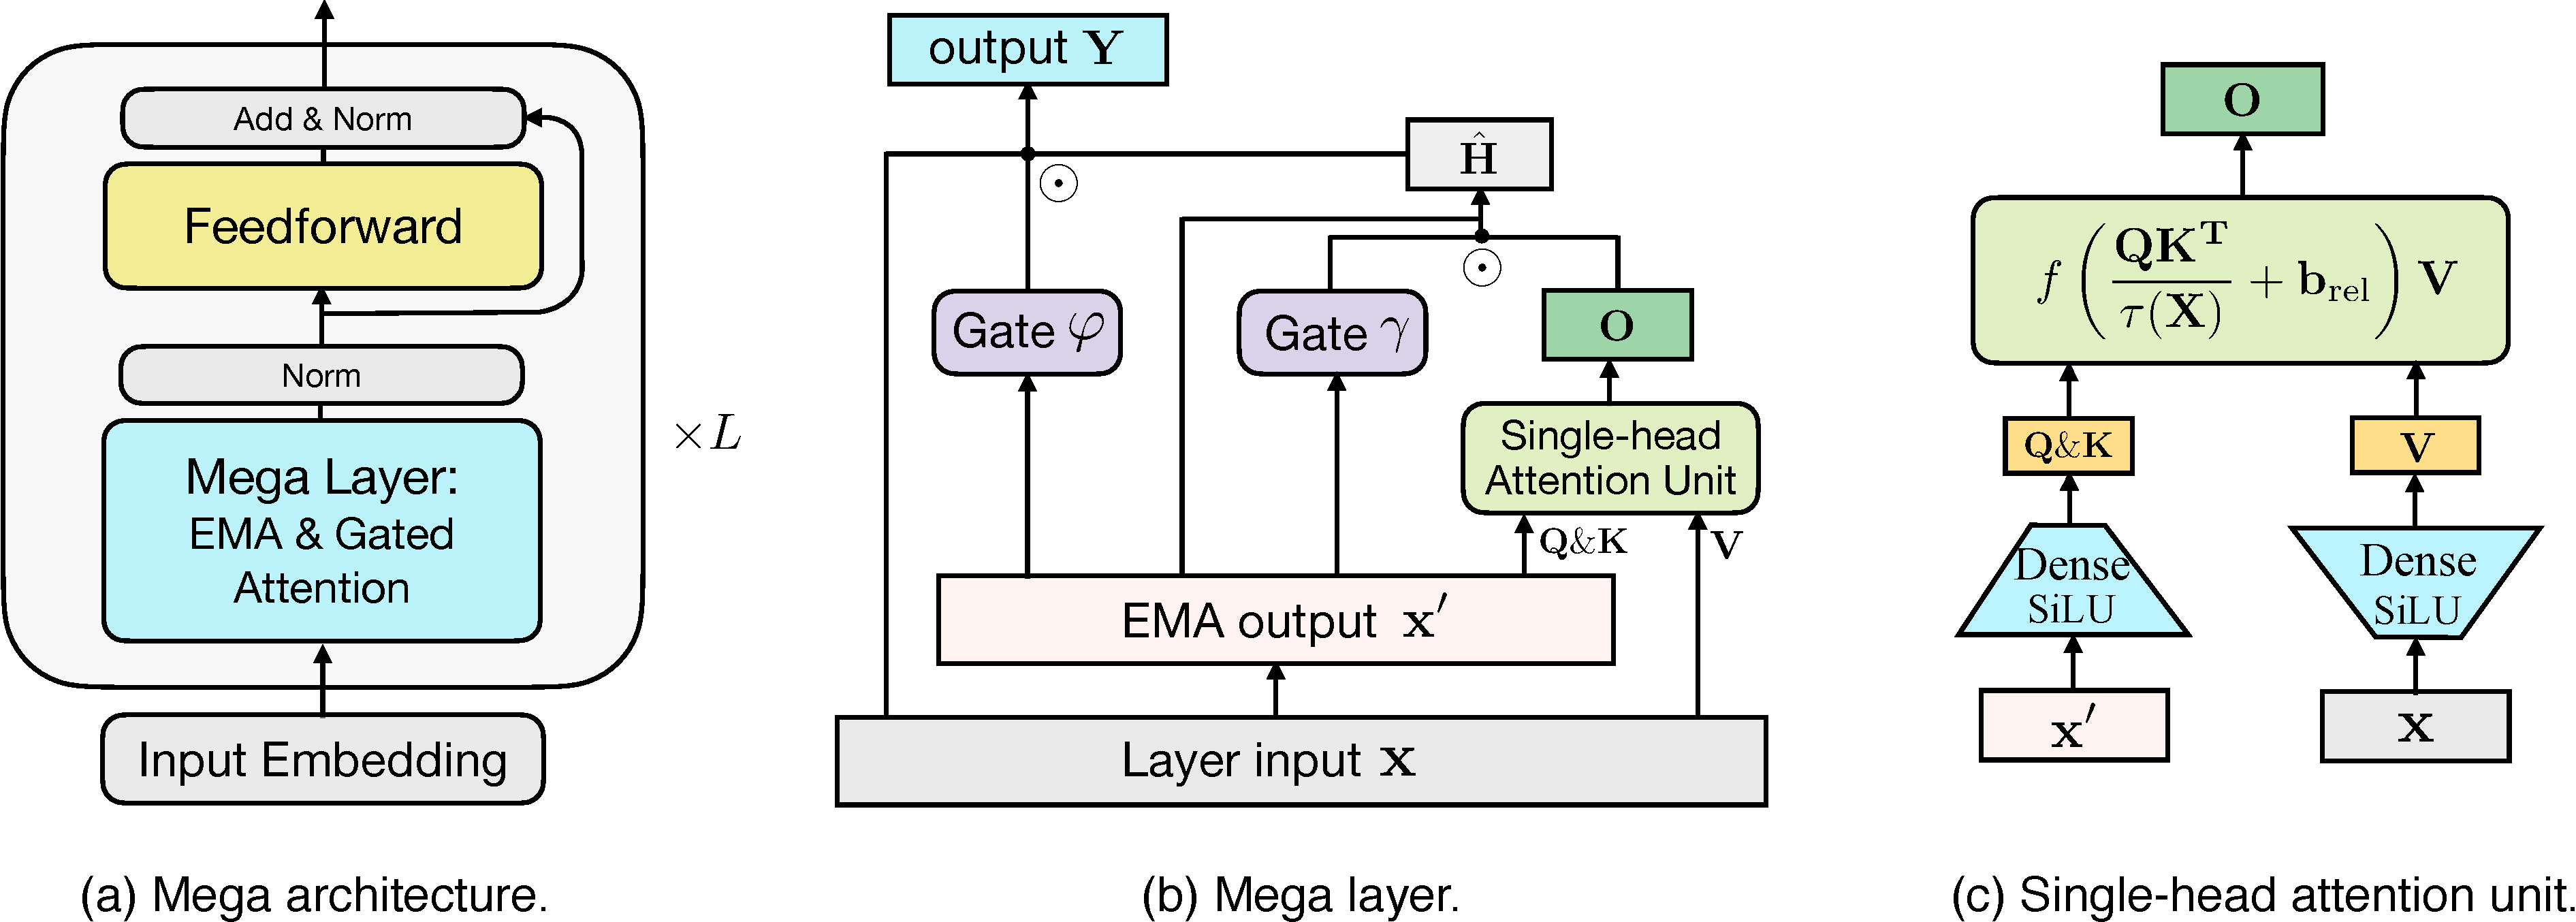
\includegraphics[width=0.99\textwidth]{figs/mega/model.pdf}
\caption{MEGA模型架构。(a) MEGA块。(b) MEGA的门控注意力层。(c) MEGA的单头注意力单元。摘自~\cite{ma2023mega}}
\label{fig:arch}
\end{figure}

\subsubs{MEGA门控注意力层}
\label{subsubsec:mega}
MEGA中的门控注意力机制采用门控循环单元(GRU\cite{cho2014properties})和门控注意力单元(GAU\cite{hua2022transformer})作为骨干结构。具体来说,首先使用\eqref{eq:mddema}中的输出计算GAU中的共享表征:
\begin{align}
\boldsymbol{X}' & = \mathrm{EMA}(\boldsymbol{X}) \qquad & \qquad \in \mathbb{R}^{n\times d} \\
\boldsymbol{Z} & = \phi_{\mathrm{silu}}(\boldsymbol{X}' W_z + b_z) \qquad & \qquad \in \mathbb{R}^{n\times z} \label{eq:z}
\end{align}
其中 $\boldsymbol{X}'$可以被视为编码了上下文信息的表征向量。而
$\boldsymbol{Z}$则是一个$z$维的高效表征。$W_z \in \mathbb{R}^{d\times z}$ 和 $b_z \in \mathbb{R}^{z}$分别是投影矩阵和偏移。
$\phi_{\mathrm{silu}}$是SiLU激活函数~\cite{ramachandran2017swish}。


在GAU之后,通过对$\boldsymbol{Z}$应用每个维度的标量和偏移量来计算查询$\boldsymbol{Q}$和键$\boldsymbol{K}$,而值序列 $\boldsymbol{V}$ 则由原始的$\boldsymbol{X}$直接得到:
\begin{align}
\boldsymbol{Q} & = \boldsymbol{\kappa}_q \odot \boldsymbol{Z} + \boldsymbol{\mu}_q \qquad & \qquad \in \mathbb{R}^{n\times z} \label{eq:query} \\
\boldsymbol{K} & = \boldsymbol{\kappa}_k \odot \boldsymbol{Z} + \boldsymbol{\mu}_k \qquad & \qquad \in \mathbb{R}^{n\times z} \\
\boldsymbol{V} & = \phi_{\mathrm{silu}}(\boldsymbol{X} W_v + b_v) \qquad & \quad \qquad \in \mathbb{R}^{n\times v} \label{eq:value}
\end{align}
这里,$\boldsymbol{\kappa}_q$、$\boldsymbol{\mu}_q$、$\boldsymbol{\kappa}_k$、$\boldsymbol{\mu}_k \in \mathbb{R}^{z}$是可学习的参数。$v$是值序列的输出维度。


注意力的计算如图~\ref{fig:arch}(c)所示,形式化表示为:
\begin{align}\label{eq:attention2}
\boldsymbol{O} & = f \left(\frac{\boldsymbol{Q}{\boldsymbol{K}}^{T}}{\tau(\boldsymbol{X})} + \boldsymbol{b}_{\mathrm{rel}} \right) \boldsymbol{V} \quad & \quad \qquad \in \mathbb{R}^{n\times v}
\end{align}
其中,$\boldsymbol{b}_{\mathrm{rel}} \in \mathbb{R}^{n\times n}$表示相对位置偏置。

类似于 GRU,MEGA引入重置门$\boldsymbol{\gamma}$、更新门$\boldsymbol{\varphi}$,并计算候选激活输出$\boldsymbol{\hat{H}}$。这些概念的含义与GRU中的概念类似。
\begin{align}
\boldsymbol{\gamma} & = \phi_{\mathrm{silu}}(\boldsymbol{X}' W_\gamma + b_\gamma) & \in \mathbb{R}^{n\times v} \label{eq:reset} \\
\boldsymbol{\varphi} & = \phi_{\mathrm{sigmoid}}(\boldsymbol{X}' W_\varphi + b_\varphi) & \in \mathbb{R}^{n\times d} \label{eq:update} \\
\boldsymbol{\hat{H}} & = \phi_{\mathrm{silu}}(\boldsymbol{X}' W_h + (\boldsymbol{\gamma} \odot \boldsymbol{O}) U_{h} + b_h) & \in \mathbb{R}^{n\times d} \label{eq:candidate}
\end{align}
输出$\boldsymbol{Y}$使用更新门$\boldsymbol{\varphi}$计算:
\begin{align}
\boldsymbol{Y} & = \boldsymbol{\varphi} \odot \boldsymbol{\hat{H}} + (1 - \boldsymbol{\varphi}) \odot \boldsymbol{X} \qquad & \qquad \in \mathbb{R}^{n\times d} \label{eq:output}
\end{align}
MEGA子层的图形架构在图~\ref{fig:arch}(b)中可视化。

\subsubs{Laplace注意力函数}
Softmax是注意力函数最常见的选择。而
\cite{so2021searching}提出的平方ReLU函数$f_{\mathrm{relu^2}}(\cdot)$在语言任务上显示出更快的收敛速度和更好的泛化性能~\cite{hua2022transformer}。
然而,$f_{\mathrm{relu^2}}(\cdot)$的一个问题是它的梯度范围没有上界这导致了模型训练不稳定。为了解决这个问题,MEGA提出了一种基于Laplace函数的新注意力函数:
\begin{equation}
\label{eq:laplace}
f_{\mathrm{laplace}}(x; \mu,\sigma) = 0.5 \times \left[1 + \mathrm{erf}(\frac{x - \mu}{\sigma\sqrt{2}}) \right]
\end{equation}
其中 $\mathrm{erf}(x) = \frac{2}{\sqrt{\pi}} \int_0^x e^{-t^2} dt$。MEGA 中,选取$\mu=\sqrt{1/2}$和$\sigma=\sqrt{1/4\pi}$ 从而使得 $f_{\mathrm{laplace}}$ 逼近 $f_{\mathrm{relu}^2}$。


\subsubs{MEGA-chunk}
\label{subsec:mega-chunk}

\begin{figure}[t]
\centering
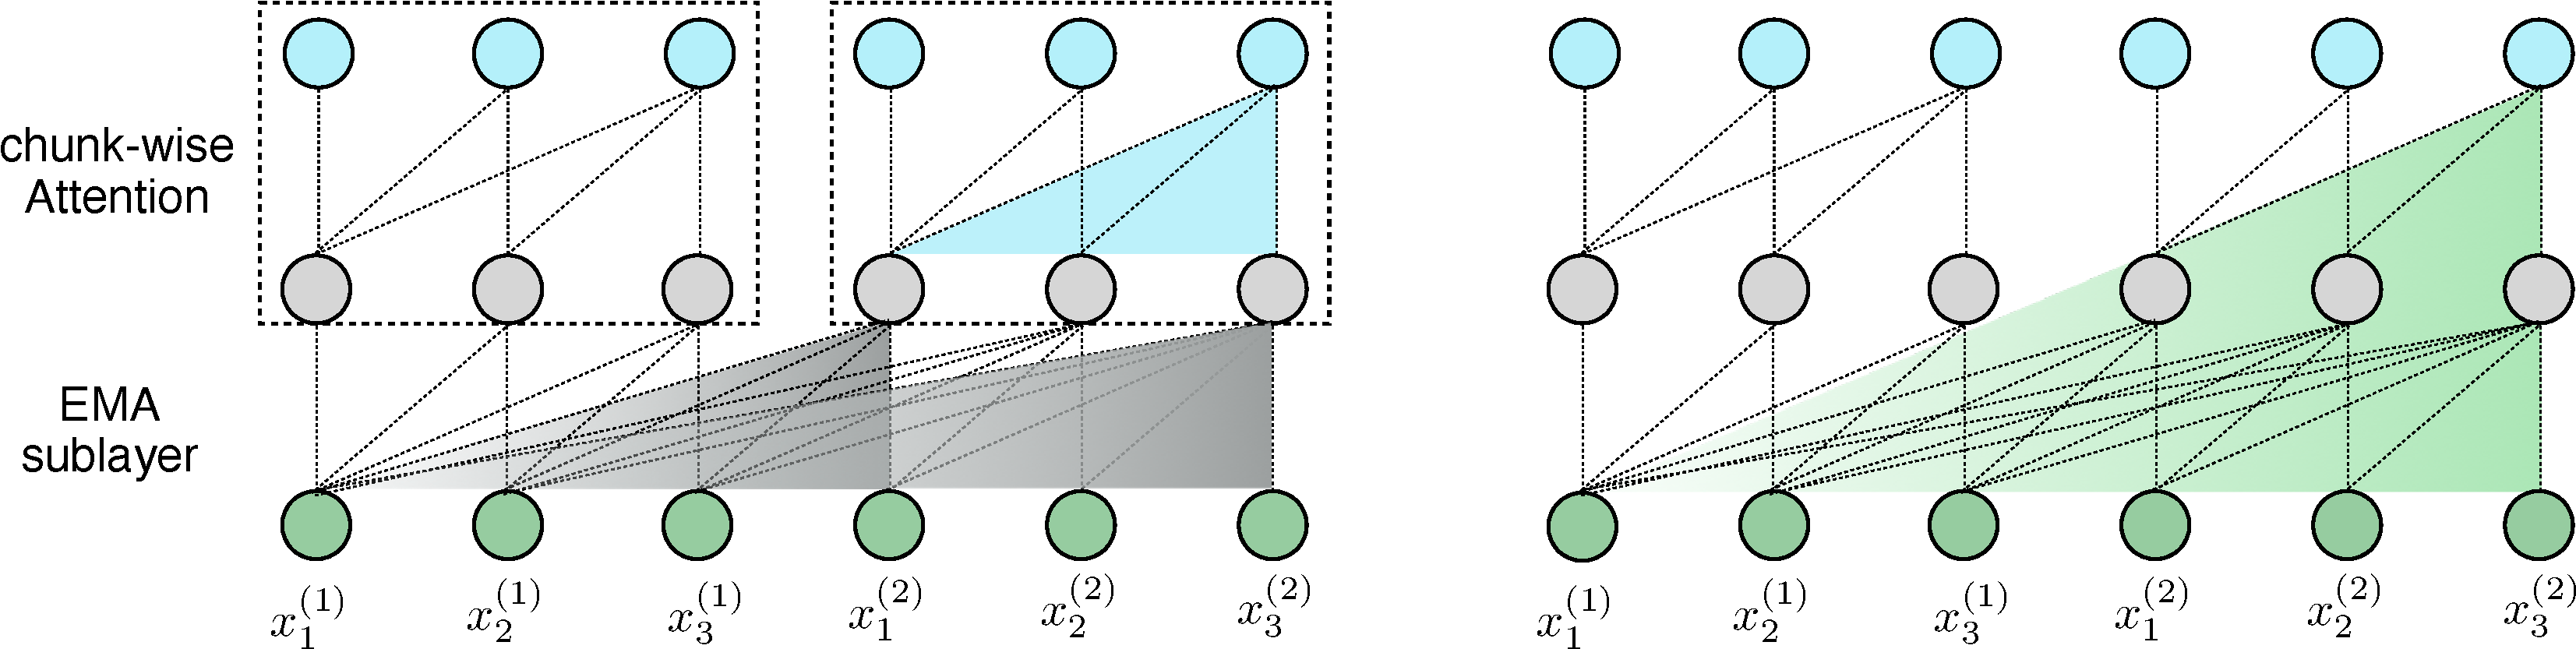
\includegraphics[width=0.99\textwidth]{figs/mega/ema_chunk_attn.pdf}
\caption{$c=3$时,MEGA-chunk 的注意力范围。摘自~\cite{ma2023mega}}
\label{fig:chunk}
\vspace{-3mm}
\end{figure}

进行了以上调整的 MEGA 注意力仍然具有$O(n^2)$ 的时空复杂度,而MEGA方法加速的关键在于将时间复杂度压缩至线性,也就是 MEGA-chunk 方法。具体来说,首先将 (\ref{eq:query}-\ref{eq:value}) 中的$\boldsymbol{Q}$, $\boldsymbol{K}$, $\boldsymbol{V}$ 序列划分为长度为 $c$ 的块,即

\begin{align}
    \boldsymbol{Q} & = \{\boldsymbol{Q}_1, \ldots,  \boldsymbol{Q}_k\} \\
    \boldsymbol{K} & = \{\boldsymbol{K}_1, \ldots,  \boldsymbol{K}_k\} \\
    \boldsymbol{V} & = \{\boldsymbol{V}_1, \ldots,  \boldsymbol{V}_k\} 
\end{align}

其中 $k = \lceil \frac n c \rceil$ 是块的数量。

接下来,每个分块独立进行\eqref{eq:attention2}中的注意力操作。这样整体的注意力复杂度对 $n$ 呈线性,即 $O(kc^2)=O(nc)$。由于在进行分块注意力前,每个时序向量通过 EMA 层捕获了块外的信息,这使其信息收集范围远超一个块的约束范围。如图~\ref{fig:chunk}所示。